\documentclass[12pt]{article}

\usepackage{amsmath}
\usepackage{amssymb}
\usepackage{geometry}
\usepackage{graphicx}
\usepackage{hyperref}

\geometry{letterpaper,tmargin=1in,bmargin=1in,lmargin=1in,rmargin=1in}

\hypersetup{
colorlinks, linkcolor=blue,
}


\begin{document}

\title{Analog Electronics}
\author{Laboratory exercise 3}
\date{Fall 2016}
\maketitle

\newpage
\section{Abstract}

In this experimentation using the information that was learned through lecture, we will design and construct our first Operational Amplifier. This amplifier will be designed in Multi-Sim 13, and the majority of our calculations and testings will also be in Multi-Sim. These amplifiers we design will be have a gain of $A_v=-10$ and $A_v=-100$ respectively. Once the designed amplifier meets all the design constraints, we will construct it using the given 741 op-amp and using our work bench tools; such as our occiliscope, function generator, multimeter, and our power supply. Once the circuit is constructed we then will test its various inputs and outputs to ensure our given $Av$'s were met.

\section{Theory}

Multi-Sim is one of the most powerful tools an electrical engineer has at there disposal. By being able to create and test a circuit before spending time \& resources constructing it, we can work out problems before hand and ensure our specifications are met. By designing two amplifiers we can better understand the importance of our resistor values and there effect on our gain,$Av$.

\newpage

\section{Experimentation}




This experimentation will use two variations of the following circuit for our gain of $A_v=-10$ and $Av=-100$ respectively.

\begin{figure}[h]
	\label{amp}
	\caption{overview design of our Amplifier}
	\centering
	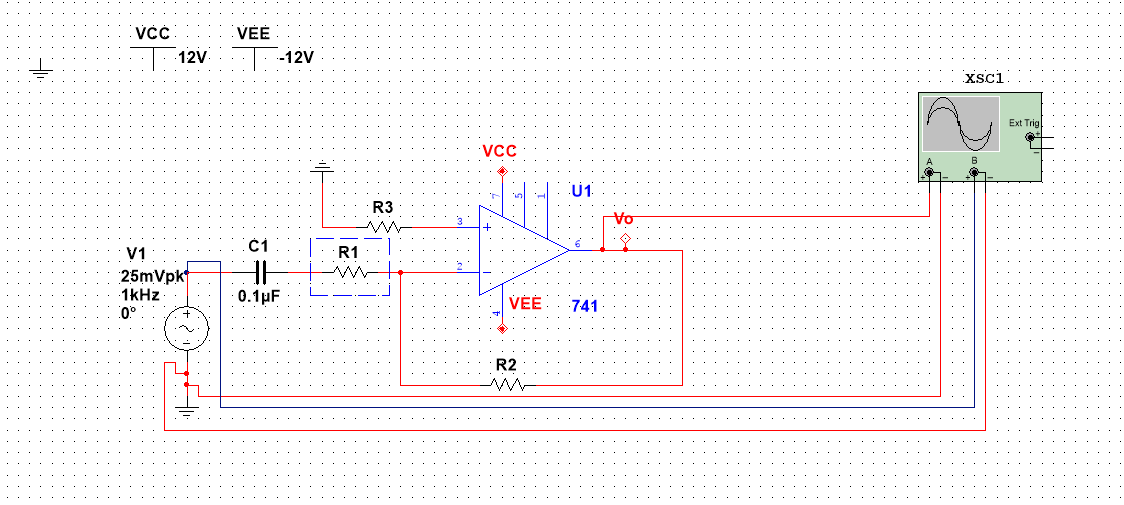
\includegraphics[width=1\textwidth]{amp}
\end{figure}

\begin{center}
	Our first circuit $A_v=-10$ will use the following resistance values
\end{center}
\begin{center}
	$R_1 =R_3= 1k\Omega$, $R_2 = 10k\Omega$
\end{center}
\begin{center}
	Our Second circuit $A_v=-100$ will use the following resistance values
\end{center}

\begin{center}
	$R_1 =R_3= 1k\Omega$, $R_2 = 100k\Omega$
\end{center}


To power our op-amp we will utilize the above schematic as reference. Do not apply voltage yet.



\newpage
\subsection{Measuring AC Gain}
\begin{enumerate}
	\item Gather a $100k\Omega$, $10k\Omega$, $.1\mu F$ capacitor, and two $1k\Omega$. Measure and log there values with the multimeter.These will be used for both circuits.
	\item Using Figure 1 and the $A_v=-10$ resistor values, place the resistors and capacitor onto the circuit board.
	\item Ensure that the resistors and capacitors go to the correct pins on our Op-Amp
	\item Power the DC voltage source on.
	\item Using the DMM measure the voltage with respect to ground of the input, output, and inverting terminals. Log this data.
	\item Attach the function generator probes to the points shown in the schematic, using the given value. Power it on.
	\item Attach the oscilloscope to the points as shown in figure 1.
	\item Measure the input and output waveforms using the oscilloscope, ensuring that DC power source is on.
	\item Log these values with your data.
\end{enumerate}

\subsection{Measuring DC gain}
Now that we measured the AC gain we can do the same for DC, to do so we must first rearrange the circuit.

\begin{enumerate}
	\item First remove the capacitor, as it will cause a short circuit when used in junction with a DC source.
	\item Replace the function generator with a $-1v$ DC voltage from the bench power supply.
	\item Using the DMM measure the output voltage from -1v to 1v on intervals of .2v
	\item Log this data into your table.
	
\end{enumerate}

For the second circuit with a gain of -100 replace the resistance values and repeat steps 2-4 in section 3.2 with a voltage of -0.1v to 0.1v by intervals of 0.02v

\newpage


\subsection{Measurements}

To calculate our gain we will compare our $V_i$ from our function generator to our $V_o$ on our oscilloscope. From these two values we can calculate the $A_v$, or gain.

$$A_v = \frac{V_o}{V_i}$$

When we plug our values in we get

$$A_v = \frac{V_o}{V_i} = \frac{830mV}{90mV} = 9.2$$

The AC gain for amplifier is $\approx 9$\\

By replace the function generator with a $-1v$ DC voltage from the bench power supply.
And using the DMM measure the output voltage from -1v to 1v on intervals of .2v, we get the following table

\begin{table}[!h]
	\centering
	\caption{$A_v=-10$}
	\label{my-label}
	\begin{tabular}{lll}
		Input Dc Voltage & Output Voltage &  \\
		-1               & 10.04          &  \\
		-0.8             & 8.03           &  \\
		-0.6             & 6.03           &  \\
		-0.4             & 4.02           &  \\
		-0.2             & 2.01           &  \\
		0                & 0.006          &  \\
		0.2              & -2             &  \\
		0.4              & -4.01          &  \\
		0.6              & -6.02          &  \\
		0.8              & -8.02          &  \\
		1                & -10.03         & 
	\end{tabular}
\end{table}
We can now calculate our DC voltage gain.
$$A_v = \frac{V_o}{V_i} = \frac{10.04V}{-1V} = 10.04$$

The DC gain for the amplifier is $\approx 10$
\newpage
By doing the same as the previous table, but with our $A_v=-100$ circuit we get this table.

\begin{table}[!h]
	\centering
	\caption{$A_v=-100$}
	\label{table 2}
	\begin{tabular}{lll}
		Input Dc Voltage & Output Voltage &  \\
		-0.1             & 10.14          &  \\
		-0.08            & 8.13           &  \\
		-0.06            & 6.11           &  \\
		-0.04            & 4.1            &  \\
		-0.02            & 2.09           &  \\
		0                & 0.081          &  \\
		0.02             & -1.9           &  \\
		0.04             & -3.9           &  \\
		0.06             & -5.98          &  \\
		0.08             & -8             &  \\
		0.1              & -10.01         & 
	\end{tabular}
\end{table}

We can now calculate our DC voltage gain.
$$A_v = \frac{V_o}{V_i} = \frac{10.1V}{-0.1V} = 101$$

The DC gain for the amplifier is $\approx 101$



\section{Conclusion}

In this experimentation we used a variety of analysis techniques to calculate and create two amplifiers that successfully took our input voltage and amplified it to a desired output voltage. During the lab several problems arouse due to my lack of experience with these circuits. The first problem was the wiring of DC power supply to both +12v and -12v. Once I understood how the DMM creates relative voltage I was able to easily fix the problem and ensure it wont happen again. Another problem I ran into was I created a fractional amplifier on accident by mixing up my $R_1$ and $R_2$ resistors. Although unintentional, it helped shape my understanding of a resistors effect on a operational amplifier. The measurements that where taking in practice although close, where not exactly what the multi-sim predicted. This is due to the fact that that Multi-sim is just that, a simulation. There are many factors that affect our reading in the real world and resistor tolerances are just one of them.


\end{document}
